
\documentclass[12pt]{article}

% including packages
\usepackage[utf8]{inputenc}
\usepackage[english]{babel}
\usepackage{amsmath}
\usepackage{graphicx}
\usepackage{wrapfig}
\usepackage[a4paper, total={6in, 8in}]{geometry}
\usepackage{hyperref}
\usepackage{hypcap}
\usepackage[autostyle]{csquotes}
\usepackage[]{biblatex}

% preferences
\graphicspath{ {images/} }
\newcommand{\lineSeparationLength}{2mm}
\hypersetup{colorlinks=true, allcolors=black}
\addbibresource{references.bib}
\ExecuteBibliographyOptions{
	giveninits=true,
	isbn=false,
	doi=false,
	url=false
}
\setlength{\parskip}{1em}

% title
\title{Using Genetic Algorithms to Find Approximations for the Minimum Vertex Cover Problem}
\author{}
\date{}





% document begins here
\begin{document}

% cover page
\pagenumbering{roman}
\cleardoublepage\phantomsection\addcontentsline{toc}{section}{Cover Page}

{
\begin{wrapfigure}{r}{0.25\textwidth}
\hfill
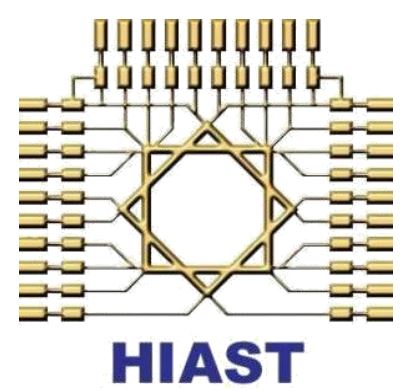
\includegraphics[width=0.9\linewidth]{hiast}
\end{wrapfigure}

\ \\[\lineSeparationLength]
Syrian Arab Republic \\[\lineSeparationLength]
Higher Institute for Applied Sciences and Technology \\[\lineSeparationLength]
Informatics Department \\[\lineSeparationLength]
Fourth Year
}

\vspace{25mm}
{\let\newpage\relax\maketitle}

\vspace{-10mm}
\begin{center}
Keywords: genetic algorithms, NP-complete, combinatorial optimization, non-deterministic algorithms, approximation algorithms, minimum vertex cover.
\end{center}

\vspace{5mm}
\begin{center}
\begin{align*}
\text{Author: }					& \textit{Farouk Hjabo} \\
\text{Academic Supervisor: }	& \textit{Dr. Said Desouki} \\
\text{General Supervisor: }		& \textit{Dr. Kadan Aljoumaa} \\
\text{Langauge Supervisor: }	& \textit{Mr. Fahmi Alammareen} \\
\end{align*}
\end{center}

\vfill
\centerline{\date{\today}}
\thispagestyle{empty}
\pagebreak

% abstract page
\cleardoublepage\phantomsection\addcontentsline{toc}{section}{Abstract}

\begin{abstract}
Lorem ipsum dolor sit amet, consectetur adipisicing elit, sed do eiusmod
tempor incididunt ut labore et dolore magna aliqua. Ut enim ad minim veniam,
quis nostrud exercitation ullamco laboris nisi ut aliquip ex ea commodo
consequat. Duis aute irure dolor in reprehenderit in voluptate velit esse
cillum dolore eu fugiat nulla pariatur. Excepteur sint occaecat cupidatat non
proident, sunt in culpa qui officia deserunt mollit anim id est laborum.
\end{abstract}

\pagebreak

% table of contents page
\cleardoublepage\phantomsection\addcontentsline{toc}{section}{Contents}
\tableofcontents
\pagebreak




% first page starts here
\pagenumbering{arabic}

\section{Introduction}
Once the NP-hardness of a combinatorial optimization
problem is established, the search for an optimal solution
is abandoned. The goal then becomes one of finding a
good heuristic, i.e. a polynomial running time algorithm
that can find solutions close to the optimal. In most cases,
traditional heuristics are problem dependent; a heuristic is
tailored to the specific problem it is trying to solve.

In this paper, we present an alternative approach that
uses genetic algorithms as a generalized heuristic for solving NP-hard combinatorial optimization problems. The
application of a genetic algorithm is demonstrated here for
the \emph{minimum vertex cover} problem. These algorithms
have been successfully applied to a broad range of problems. This wide range can be tackled by genetic algorithms
mainly due to the fact that they work with an encoding of
the domain rather than with the problem domain itself.


\section{Genetic Algorithms}
Lorem ipsum dolor sit amet, consectetur adipisicing elit, sed do eiusmod
tempor incididunt ut labore et dolore magna aliqua. Ut enim ad minim veniam,
quis nostrud exercitation ullamco laboris nisi ut aliquip ex ea commodo
consequat. Duis aute irure dolor in reprehenderit in voluptate velit esse
cillum dolore eu fugiat nulla pariatur. Excepteur sint occaecat cupidatat non
proident, sunt in culpa qui officia deserunt mollit anim id est laborum.
 

\section{The Minimum Vertex Cover Problem}
Lorem \cite{einstein} ipsum dolor sit amet, consectetur adipisicing elit, sed do eiusmod
tempor incididunt ut labore et dolore magna aliqua. Ut enim ad minim veniam,
quis nostrud exercitation ullamco laboris nisi ut aliquip ex ea commodo
consequat. Duis aute irure dolor in reprehenderit in voluptate velit esse
cillum dolore eu fugiat nulla pariatur. Excepteur sint occaecat cupidatat non
proident, sunt in culpa qui officia deserunt mollit anim id est laborum.


\section{Experimental Results}
Lorem \cite{dirac} ipsum dolor sit amet, consectetur adipisicing elit, sed do eiusmod
tempor incididunt ut labore et dolore magna aliqua. Ut enim ad minim veniam,
quis nostrud exercitation ullamco laboris nisi ut aliquip ex ea commodo
consequat. Duis aute irure dolor in reprehenderit in voluptate velit esse
cillum dolore eu fugiat nulla pariatur. Excepteur sint occaecat cupidatat non
proident, sunt in culpa qui officia deserunt mollit anim id est laborum.


\section{Conclusion}
Lorem \cite{ctan} ipsum dolor \cite{khuri1994evolutionary}
sit amet, consectetur adipisicing elit, sed do eiusmod
tempor incididunt ut labore et dolore magna aliqua. Ut enim ad minim veniam,
quis nostrud exercitation ullamco laboris nisi ut aliquip ex ea commodo
consequat. Duis aute irure dolor in reprehenderit in voluptate velit esse
cillum dolore eu fugiat nulla pariatur. Excepteur sint occaecat cupidatat non
proident, sunt in culpa qui officia deserunt mollit anim id est laborum.


\pagebreak


\cleardoublepage\phantomsection\addcontentsline{toc}{section}{References}
%\bibliographystyle{abbrv}
%\bibliography{references}
\printbibliography

% end of document
\end{document}


